\chapter{Dataset and Data Representation}
\paragraph{Overview}
This chapter aims to be a description of the dataset structure the model is trained and evaluated with, as well as an overview of the processes that led to the creation of the dataset themselves.
In section~\ref{sec:Sources} a reference to the data sources is given, then the focus of section~\ref{sec:WAD} will be on how data is natively encoded for the game engine in order to give some hints on what are the difficulties to face in converting to and from that format in an automatic way. Section~\ref{sec:TargetFormat} will describe in detail what data is provided with the dataset and how levels are converted from the native format and what features are extracted in order to provide an input for the neural network. Lastly, section~\ref{sec:DatasetOrganization} will give an overview of how the data is provided and organized in the resulting dataset.
 
\section{Data Sources}
\label{sec:Sources}
\paragraph{Archive} All data used to train and validate the model comes solely from the \textit{Idgames Archive} founded in 1994 by Barry Bloom \cite{idarchivehistory} and mirrored on various FTP sources. The mirror we used for collecting levels is Doomworld.com \cite{url:doomworld} which is one of the oldest and currently most active community about the DOOM video-game series \cite{wiki:doomworld}.
\paragraph{Level Selection} Idgames archive includes levels for multiple games such as DOOM, DOOM 2 or their various modifications and they are divided in hierarchical categories which classifies levels by game, game mode (multi-player "deathmatch" or single-player), and alphabetically.
Amongst all the categories we selected only those levels that belong to "doom" and "doom2" excluding sub-categories named "deathmatch" and "Ports". This choice has been made in order to avoid mixing possibly different kinds of levels, since a level designed for a Single Player Mode could be structurally different from a level which is designed for multi-player games. Moreover the "Ports" category has been excluded because levels contained in it are intended to work with modifications of the game engine code and it would have led to problems in managing every particular exceptional behaviour.

\paragraph{Source Data Organization} Levels in Idgames archive are stored in zip archives including a "READ ME" text file containing author notes and the \gls{WAD} file that contain up to 32 levels. 
Each zip archive can be downloaded from the respective download page which presents a variable quantity of information such as the author, a short description, screen shots, user reviews, number of views and downloads, etc.
The dataset we present in this work always keeps track of these information about each level for correct attribution and also offers a "snapshot" of average user review score and the number of views and downloads when available. It is worth noting that since Doomworld website recently switched to a different download system \cite{wiki:doomworld}, data may not always be accurate, especially those concerning download and view counts, but they are still proposed as a starting point for further research. 
\section{Source Data Format: WAD Files}
\label{sec:WAD} 
\paragraph{Introduction} The Doom Game Engine \cite{doomengine} makes use of package files called "\glspl{WAD}" to store every game resource such as Levels, Textures, Sounds, etc. 
\gls{WAD} files have been designed in order to make the game more extendible and customizable and opened the way for a considerably large amount of user-generated content. This section is not meant to be a complete description of how \glspl{WAD} files are structured but only an overview of which aspects we considered for writing the software that generates the dataset from the \gls{WAD} files. Every information about \glspl{WAD} files has been taken from the \citetitle{doomspecs} \cite{doomspecs} and we demand to that document a deeper explanation on every aspect of the file format.
\subsection{Overview}
\paragraph{Type of WADs}
\glspl{WAD} are of two types, called "IWAD" or "Internal WAD" and "PWAD" or "Patch WAD". The original game \glspl{WAD}, called "DOOM.WAD" and "DOOM2.WAD", are of the "IWAD" type as they contain every asset that is needed for the game to run, while all the \glspl{WAD} containing custom content or modifications to existing content are of the "PWAD" type. The content which is defined in a PWAD is added or replaced to the original IWAD when the \gls{WAD} is loaded, for example if a PWAD defines the level "MAP01", which is already defined in "DOOM2.WAD", the PWAD level is loaded instead of the original one, while maintaining all the other content unaltered.
Since in our work we deal only with PWADs, we will generally refer to them simply as \glspl{WAD}.

\paragraph{Lumps} Every data inside a \gls{WAD} is stored as a record called \gls{lump} which has a name up to 8 characters and a structure and size which is different depending on the lump type. In general there are no restrictions on lump order with the exception of some of them, including Lumps needed for defining a Level.

\paragraph{WAD Structure} Every \gls{WAD} file is divided in three sections: A header, a set of \glspl{lump} and a trailing Directory. The header holds the information about the WAD type, the number of \glspl{lump} and the location of the Directory, which is positioned after the last \gls{lump}. The directory contains one 12-bytes entry for each \glspl{lump} included in the file that specifies the \glspl{lump} location, size and name. Table~\ref{tab:WADStructure} reports a simplified description of a \gls{WAD} file.



\begin{table}[b]
	\centering
	\begin{tabularx}{\textwidth}{| c | c | c | c | X | }
		\hline
		Section Length (bytes) & Section Name & Field Size & Field Name & Description \\
		\hline
		   &   & 4 & Identification & ASCII string "PWAD" or "IWAD" \\ \cline{3-5}
		12 &     Header			  & 4 & Number of Lumps & The number of Lumps included in the WAD \\  \cline{3-5}
		&   						  & 4 & Table Offset & Integer pointer to the Dictionary \\ \cline{3-5}
		\hline
		Variable& Lumps & - & Lump Data & Lumps stored as a stream of Bytes \\
		\hline
		&                              & 4 & Lump Position & Integer holding a point to the lump's data \\ \cline{3-5}
		16 * Number of Lumps  & \multirow{3}{*}{}{Directory} & 4 & Lump Size & Size of the lump in bytes \\ \cline{3-5}
		&                              & 8 & Lump Name & Lump name in ASCII, up to 8 bytes long. Shorter names are null-padded \\ \cline{3-5}
		\hline
	\end{tabularx}
\caption{WAD File structure}
\label{tab:WADStructure}
\end{table}

\paragraph{Coordinate Units} \label{par:coords} The Doom game engine describes coordinates using integer values between -32768 and +32767 and it is proportional to one pixel of a texture. This unit is called "Map Unit" or "Doom Unit" in this work. Although there's not an unique real world interpretation of one Map Unit, we used an approximation for which each relevant map tile or image pixel is 32x32 MU large; this choice is motivated by the fact that the smallest radius of a functional object in DOOM is 16 MU. 

\newpage

\subsection{Doom Level Format}
\paragraph{Overview} Level data in a \gls{WAD} file follows a precise structure. In particular each level is composed of an ordered sequence of lumps that describes the its structure:
	\begin{description}[wide=\parindent]
		\item[(NAME)]: Name of the level slot in DOOM or DOOM2 format.
		\item[THINGS] List of every game object ("\gls{thing}") that is placeable inside the level.
		\item[LINEDEFS] List of every line that connects two vertices.
		\item[SIDEDEFS] A list of structures describing the sides of every Linedef.
		\item[VERTEXES] Unordered list of vertices.
		\item[SEGS] A list of linedef segments that forms sub-sectors.
		\item[SSECTORS] A list of sub-sectors, which are convex shapes forming sectors.
		\item[NODES] A binary tree sorting sub-sectors for speeding up the rendering process.
		\item[SECTORS] A list of Sectors. A \gls{sector} is a closed area that has the same floor and ceiling height and textures.
		\item[REJECT] Optional lump that specifies which sectors are visible from the other. Used to optimize the AI routines.
		\item[BLOCKMAP] Pre-computed collision detection map. 
	\end{description}

\paragraph{Essential Subset and Optimizations} It is important to notice that although all the lumps above (with the exception of REJECT) are mandatory to build a playable level, some of them can be automatically generated from the remaining ones using external tools. In particular an editor software or designer has to provide at least the lumps (name), THINGS, LINEDEFS, SIDEDEFS, VERTEXES and SECTORS. The lumps SEGS, SSECTORS, NODES, REJECT and BLOCKMAP serve the purpose of speeding-up the rendering process by avoiding runtime computation. In particular the Doom Engine uses a Binary Space Partitioning Algorithm \cite{Fuchs:1980:VSG:965105.807481} for pre-computing the Hidden surface determination (or occlusion culling) and it is usually done by an external tool. In this work we used the tool "\citetitle{bsp}" \cite{bsp} in the last stage of the pipeline in order to produce playable DOOM levels from the network output. In the following paragraphs only the lump types that are not generated by the external tool are described.

\paragraph{(Name)} The first lump of a level is its slot name. We indicate this lump between parenthesis because differently from the other lumps, this one has no data associated but the Name field in the Directory is the slot name itself and the size is therefore zero. The level name descriptor has to match either \textit{ExMy} ("Episode x, Map y") or \textit{MAPzz} for DOOM or DOOM2 respectively, where x ranges from 1 to 4, y from 1 to 9 and zz from 1 to 32.


\paragraph{Things} A doom "\gls{thing}" is every object included in a level that is not a wall, pavement, or a door. A "Things" lump is a list of entries each one containing five integers specifying the \textit{position} (x,y) in \gls{MU}, the \textit{angle} the thing is facing the \textit{Thing type} index and a set of flags indicating in which difficulty level the thing is present and if the thing is deaf if it is an enemy.

\paragraph{Linedefs} A \gls{linedef} is any line that connects two vertices. Since DOOM maps are actually bi-dimensional, a single line is needed to define each wall or step. \glspl{linedef} do not necessarily have to match with visible entities, as each \gls{linedef} can also represent invisible boundaries or triggers, which can be thought as tripwires or switches that make something happen to a sector. If the \gls{linedef} acts as a trigger than it references another sector and has a type which defines what would happen to it when the \gls{linedef} is activated. For example a door is implemented as a sector that raises up to the ceiling when a certain \gls{linedef} is triggered, but this behaviour is specified in the switch and not in the door as one might think. All the options are defined by a set of flags that specifies what kind of objects the \gls{linedef} blocks, if it's two sided or not, the trigger activation condition and so on.
Finally, each \gls{linedef} has to specify what "vertical plane" (or \gls{sidedef}) lies on its right and left side. Only the "left sidedef" field can be left empty, due to the way the sectors are represented.

\paragraph{Sidedefs} A \glossary{sidedef} is a structure that contains the texture data for each linedef. It corresponds to the side of each wall and it's referenced by the linedefs. Other than the options for texture visualization it also specifies the sector number that this plane is facing, implicitly defining the sector boundaries.

\paragraph{Vertexes}\footnote{Although the correct spelling should be "vertices", we keep the original version of the field name.} This is the simplest kind of \gls{lump}, consisting in an unordered list of map coordinates, in \gls{MU}. Each entry has an x and y position expressed in a 16-bit signed integer. \glspl{linedef} references the starting and ending vertex by reporting their index in this list.

\paragraph{Sectors} A sector is defined as any area that have constant floor and ceiling heights and textures. This definition highlights the fact that the doom engine is in fact a 2d engine, since it's not possible to define a sector above or below another one. A sector does not necessarily have to be closed nor a single connected polygon, but non-closed sectors can cause some issues during gameplay. The only constraint to define sectors comes from the fact that linedefs must have a right sidedef but the left one is optional, which means that the sectors are normally described as (a set of) positively oriented curves \cite{poly_orient} with the exception of linedefs that are shared with another sector, that may be reversed. The fields of a sector lump includes the floor and ceiling height, the name of the floor and ceiling texture, the light level, the "type" to controls some lighting effects and damaging floor, and the tag number that is referenced by the linedef triggers. Figure~\ref{fig:sectors} shows an example of a level with 3 sectors.


\begin{figure}
	\begin{center}
		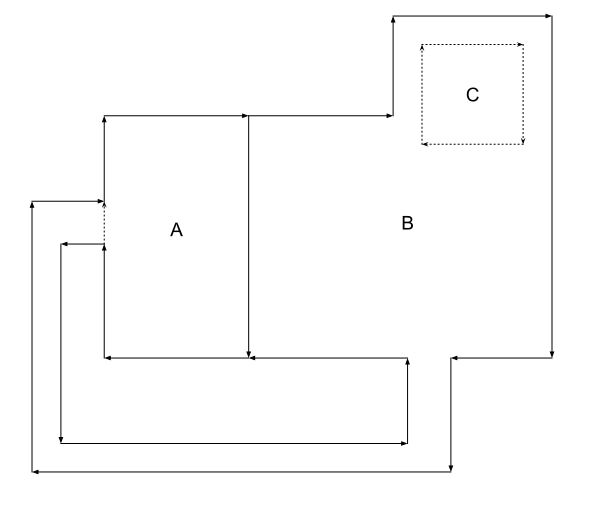
\includegraphics[width=0.8\linewidth]{linedefs_and_sectors}
	\end{center}
	
	\captionsetup{width=0.8\linewidth}
	\caption[A simple level showing sectors and linedefs]{A simple level showing three sectors A, B and C and the linedefs defining them, following the positive oriented curve constraint. Sector C can be viewed as a small platform inside the sector B. Solid arrows represent walls, while dashed lines represent invisible linedefs or changes in height between two sectors (steps). In this level, every solid arrow is a linedef that specifies only a right sidedef, with the exception of the one separating sectors A and B that has both a right and a left one.}
	\label{fig:sectors}
	\medskip
	
\end{figure}


\subsection{Conversion issues} 
Since 1994 many DOOM players started producing a large amount of levels and increasingly sophisticated editors came to light. This led to a notable variety in conventions, optimizations and use of bad practices that we tried to deal with in developing the Python module for reading and writing wad files. Some of these practices includes unnecessary lumps, random-data instead of null padding for names and other inconsistencies or arbitrary conventions. 
However, we paid particular attention during the writing phase in order to precisely follow the specifications and avoid generating low quality WAD files as much as we could.
Some other difficulties came with the necessity to render wad files as images and vice-versa. The first one is that neither \glspl{linedef} nor vertices came in an any ordered format, along with the fact that sector vertices are not explicitly defined but only referenced through the linedef/sidedef chain which means that for finding a sector shape one has to find all sidedefs with the desired sector number, than find all the linedefs referencing those sidedefs and lastly retrieving the vertices, leading to an increase of complexity. Another one is given by the fact that although sectors must be positively oriented curves, it is not mandatory to use the left sidedefs for adjacent sectors, leading to duplicated linedefs in the opposite direction. Even some optimizations such as sidedef compression may be possible, that is referencing the same sidedef wherever the same wall texture is used, adding complexity to the conversion script. Lastly, the concept of sector and the concept of room are not equivalent, since even though a sector is defined as an area of constant height this does not enforce to define a sector only where height changes, so the semantic of a sector actually depends on the designer and the editor used. 


\section{Target Data Format: Feature Maps and Vectors}
\label{sec:TargetFormat}
\paragraph{Introduction} This section provides a description of the data format as it is stored in the level dataset.
\subsection{Level Description and Motivation}
%TODO: Perché le immagini? Come mai divise così? Come mai l'encoding in questo modo?
\paragraph{}Levels are read as a structured object by a module we wrote for the purpose of providing developers and designers a programmatic way to access, analyse and edit DOOM WAD files, instead of using visual authoring software. This allows to automatise some tasks that would be very long to accomplish with standard editors or tools and also offers developers the possibility to write custom editor and scripts. \\*
In order to provide the most complete set of information possible every level is converted to a set of images, called \glspl{featuremap} in this work, a tiled representation in textual format that is an extension of the one taken from \cite{VGLC}, a graph representation and a set of textual and scalar features that contains both the \gls{WAD} meta-data and the level features and metrics calculated either on the WAD representation (sectors, subsectors, linedefs, etc), the \gls{featuremap} representation or the graph representation of the level. A detailed list and explanation of each feature is provided in section~\ref{features}. \\*
The choice of these representations have been made primarily for the need of having a data format that the generator model can work  on. In particular, convolutional neural netoworks are naturally designed to work well with bi-dimensional or tri-dimensional data such as (multi-channel) images, for this reason the image representation arose naturally. The text representation is provided mainly for consistency with the data format given in \cite{VGLC}, even if our representation uses two characters per tile instead of one. Finally, scalar and graph representation have been collected for the need of quantifying and summarising some properties and having a more abstract representation of a level, which can be very helpful in the case this data had to be used in other works.

\subsection{Feature Maps}
%TODO: Describe the maps and data encoding
\paragraph{} \glspl{featuremap} are a set of images each of them describing a different aspect of the level. In particular we used for each \gls{featuremap} a grayscale 8-bit image in which each pixel can assume values between 0 an 255. This allowed to obtain a good degree of precision while still maintaining a reasonable dataset size. \\*
Because of the motivations explained in section~\ref{par:coords}, each pixel in a \gls{featuremap} corresponds to a square of 32x32 \gls{MU}. 
In the following paragraph we will describe in detail each of them along with the data encoding.

\paragraph{\gls{floormap}} The \gls{floormap} is the most basic form of level representation, since it only represents which part of the space are occupied by the level and which are empty. This kind of map is often used in robotic mapping. \\*
This map also describes approximatively the level area that is possible to traverse, since in DOOM walls have no thickness. \\*
"Floor" pixels have value 255 (white) and "Empty" pixels have value 0 (black).

\paragraph{\gls{wallmap}} The \gls{wallmap} represent the impassable walls of the level. They are represented as a one-pixel-wide line and are obtained by directly drawing each \gls{linedef} with the impassable flag set on a black image. \\*
Pixel values are 0 for Empty area or floors and 255 for the walls.

\paragraph{\gls{heightmap}} The \gls{heightmap} is another common map used for visualizing the height of a certain surface. Since height level in DOOM levels are completely arbitrary and virtually unbounded, we normalize each level between its lowest and highest height, assigning the pixel value 0 for empty parts of the level and the remaining are calculated from the formula $ c_{h} = \lfloor h * \dfrac{255}{|H|} \rfloor $, where $ H $ is the ordered set of possible height values for the level and $ h \in \{1, 2, ..., |H| \} $ is the index of the height value in $ H $ for which we want to calculate the encoded colour. \\*
 For example if a level takes the height values $ H = \{ 0, 10, 15, 20 \} $ they will be encoded respectively as $ c_{h} = \{ 63, 127, 191, 255\} $ and 0 for the empty areas. Although this map loses the information about the differences between a height level and another, it has the advantage to represent "higher" and "lower" parts of the level without polarizing the entire map due to extreme levels: while the majority of the levels has a few changes that can be approximated as uniform (such as levels with stairs connecting a few rooms), other had some extreme changes in height but only for a small portion of the map (like a very high elevator leading to a small secret room) that led to scaling problems.
 
\paragraph{\gls{thingsmap}} The \gls{thingsmap} represent only data that is contained in the THINGS lump. It features a series of pixels placed at the thing coordinate, with a value that corresponds to a particular "thing". Pixel colours have been grouped by functional purposes so for example weapons occupies values that are close each other. This is for tolerating some output noise during generation without completely changing the functional aspect of an object as would have happened if we kept the original things encoding. Tables \ref{tab:thingsmap1}, \ref{tab:thingsmap2} and \ref{tab:thingsmap3} lists the complete encoding for the maps. Descriptions are taken from \cite{wiki:thingtypes}.

\begin{table}[b]
	\centering
	\begin{tabularx}{\textwidth}{| c | c | X | }
		\hline
		Value & Functional Category & Thing Description \\
		\hline
		0	& 	& Empty \\
		1	& other	& Boss Brain \\
		2	& other	& Deathmatch start \\
		3	& other	& Player 1 start \\
		4	& other	& Player 2 start \\
		5	& other	& Player 3 start \\
		6	& other	& Player 4 start \\
		7	& other	& Spawn shooter \\
		8	& other	& Spawn spot \\
		9	& other	& Teleport landing \\
		10	& keys	& Blue keycard \\
		11	& keys	& Blue skull key \\
		12	& keys	& Red keycard \\
		13	& keys	& Red skull key \\
		14	& keys	& Yellow keycard \\
		15	& keys	& Yellow skull key \\
		16	& decorations	& Bloody mess \\
		17	& decorations	& Bloody mess \\
		18	& decorations	& Candle \\
		19	& decorations	& Dead cacodemon \\
		20	& decorations	& Dead demon \\
		21	& decorations	& Dead former human \\
		22	& decorations	& Dead former sergeant \\
		23	& decorations	& Dead imp \\
		24	& decorations	& Dead lost soul (invisible) \\
		25	& decorations	& Dead player \\
		26	& decorations	& Hanging leg \\
		27	& decorations	& Hanging pair of legs \\
		28	& decorations	& Hanging victim, arms out \\
		29	& decorations	& Hanging victim, one-legged \\
		30	& decorations	& Hanging victim, twitching \\
		31	& decorations	& Pool of blood \\
		32	& decorations	& Pool of blood \\
		33	& decorations	& Pool of blood and flesh \\
		34	& decorations	& Pool of brains \\
						\hline
			\end{tabularx}
		\caption{ThingsMap Encoding (1 of 3)}
		\label{tab:thingsmap1}
		\end{table}
		
		\begin{table}[b]
			\centering
			\begin{tabularx}{\textwidth}{| c | c | X | }
				\hline
				Value & Functional Category & Thing Description \\
				\hline
		
		35	& obstacles	& Barrel \\
		36	& obstacles	& Burning barrel \\
		37	& obstacles	& Burnt tree \\
		38	& obstacles	& Candelabra \\
		39	& obstacles	& Evil eye \\
		40	& obstacles	& Five skulls "shish kebab" \\
		41	& obstacles	& Floating skull \\
		42	& obstacles	& Floor lamp \\
		43	& obstacles	& Hanging leg \\
		44	& obstacles	& Hanging pair of legs \\
		45	& obstacles	& Hanging torso, brain removed \\
		46	& obstacles	& Hanging torso, looking down \\
		47	& obstacles	& Hanging torso, looking up \\
		48	& obstacles	& Hanging torso, open skull \\
		49	& obstacles	& Hanging victim, arms out \\
		50	& obstacles	& Hanging victim, guts and brain removed \\
		51	& obstacles	& Hanging victim, guts removed \\
		52	& obstacles	& Hanging victim, one-legged \\
		53	& obstacles	& Hanging victim, twitching \\
		54	& obstacles	& Impaled human \\
		55	& obstacles	& Large brown tree \\
		56	& obstacles	& Pile of skulls and candles \\
		57	& obstacles	& Short blue firestick \\
		58	& obstacles	& Short green firestick \\
		59	& obstacles	& Short green pillar \\
		60	& obstacles	& Short green pillar with beating heart \\
		61	& obstacles	& Short red firestick \\
		62	& obstacles	& Short red pillar \\
		63	& obstacles	& Short red pillar with skull \\
		64	& obstacles	& Short techno floor lamp \\
		65	& obstacles	& Skull on a pole \\
		66	& obstacles	& Stalagmite \\
		67	& obstacles	& Tall blue firestick \\
		68	& obstacles	& Tall green firestick \\
		69	& obstacles	& Tall green pillar \\
		70	& obstacles	& Tall red firestick \\
		71	& obstacles	& Tall red pillar \\
		72	& obstacles	& Tall techno floor lamp \\
		73	& obstacles	& Tall techno pillar \\
		74	& obstacles	& Twitching impaled human \\
		
								\hline
	\end{tabularx}
\caption{ThingsMap Encoding (2 of 3)}
\label{tab:thingsmap2}
\end{table}

\begin{table}[b]
\centering
\begin{tabularx}{\textwidth}{| c | c | X | }
\hline
Value & Functional Category & Thing Description \\
\hline
		
		75	& monsters	& Arachnotron \\
		76	& monsters	& Arch-Vile \\
		77	& monsters	& Baron of Hell \\
		78	& monsters	& Cacodemon \\
		79	& monsters	& Chaingunner \\
		80	& monsters	& Commander Keen \\
		81	& monsters	& Cyberdemon \\
		82	& monsters	& Demon \\
		83	& monsters	& Former Human Trooper \\
		84	& monsters	& Former Human Sergeant \\
		85	& monsters	& Hell Knight \\
		86	& monsters	& Imp \\
		87	& monsters	& Lost Soul \\
		88	& monsters	& Mancubus \\
		89	& monsters	& Pain Elemental \\
		90	& monsters	& Revenant \\
		91	& monsters	& Spectre \\
		92	& monsters	& Spider Mastermind \\
		93	& monsters	& Wolfenstein SS \\
		94	& ammunitions	& Ammo clip \\
		95	& ammunitions	& Box of ammo \\
		96	& ammunitions	& Box of rockets \\
		97	& ammunitions	& Box of shells \\
		98	& ammunitions	& Cell charge \\
		99	& ammunitions	& Cell charge pack \\
		100	& ammunitions	& Rocket \\
		101	& ammunitions	& Shotgun shells \\
		102	& weapons	& BFG 9000 \\
		103	& weapons	& Chaingun \\
		104	& weapons	& Chainsaw \\
		105	& weapons	& Plasma rifle \\
		106	& weapons	& Rocket launcher \\
		107	& weapons	& Shotgun \\
		108	& weapons	& Super shotgun \\
		109	& powerups	& Backpack \\
		110	& powerups	& Blue armor \\
		111	& powerups	& Green armor \\
		112	& powerups	& Medikit \\
		113	& powerups	& Radiation suit \\
		114	& powerups	& Stimpack \\
		115	& artifacts	& Berserk \\
		116	& artifacts	& Computer map \\
		117	& artifacts	& Health potion \\
		118	& artifacts	& Invisibility \\
		119	& artifacts	& Invulnerability \\
		120	& artifacts	& Light amplification visor \\
		121	& artifacts	& Megasphere \\
		122	& artifacts	& Soul sphere \\
		123	& artifacts	& Spiritual armor  \\
		\hline
	\end{tabularx}
	\caption{ThingsMap Encoding (3 of 3)}
	\label{tab:thingsmap3}
\end{table}

\paragraph{\gls{triggermap}} The \gls{triggermap} is used for representing linedef triggers and the sectors which activates. Due to the vast amount of cases the doom engine can handle, only a few types of triggers have been considered. The mapping works by assigning an integer $ i \le 32 $ to every trigger object, and subdividing triggers types in 5 groups: local doors (the ones that are activable only if the players directly interact with them), remote doors, lifts, switches and teleports. Local doors can be normal or require a key of a certain colour in order to open, but they are not indexed by the trigger index since they don't require to be linked to other linedefs in order to be opened. Table~\ref{tab:triggermap} describes the encoding for each possible item $ i $.

\begin{table}[h]
\begin{tabularx}{\textwidth}{| c | c | X | }
	\hline
	Value & Functional Category & Thing Description \\
	\hline
	0 &	None &	Empty \\
	10 &	local doors	 & Blue key local door \\
	12 &	local doors & Red key local door \\
	14 &	local doors	 & Yellow key local door \\
	16 &	local doors & Local door \\
	32+i &	remote doors &	Remote door with tag i \\
	64+i &	lifts &	Lift with tag i \\
	128+i &	switch &	Linedef that activates the i tag \\
	192+i &	teleports &	teleport to sector i \\
	255 &	exit &	Level Exit \\
	\hline
\end{tabularx}
\caption[TriggerMap Encoding]{TriggerMap Encoding: Each item i is connected to one or more objects. For example: switch (128+1) will open the door (32+1), raise the lift (64+1), etc.}
\label{tab:triggermap}
\end{table}

\paragraph{\gls{roommap}} The \gls{roommap} represent an enumeration of the rooms obtained with an algorithm that is very similar to the morphological approach used in \citetitle{7487234}\cite{7487234}: An euclidean distance transform \cite{edt} is first applied to the \gls{floormap} obtaining a map that we call \"Distance Map\" or \"DistMap\", then the local maxima are found \cite{localmax} such that each maximum has a minimum distance of 3 from the closest one, resulting in the room center coordinates that are used as markers for a Watershed segementation \cite{watershed} using the negative distance map as basin. This results in a room segmentation that is good enough for descriptive purposes while maintaining good performances.

\subsection{Graph Representation}
Another way to represent the level is by using a graph. In particular, this graph is a region adjacency graph \cite{Trémeau00regionsadjacency} built upon the \gls{roommap}, where the nodes represent the rooms and the edges are the boundaries they have in common. This graph is built primarily for computing some features about the level and for exploiting its convenient representation of the rooms during the WAD Writing phase: this graph can be annotated with the coordinates of walls belonging to each room, and this information can be used to build a level room-by-room, with the assumption that a room could approximate a sector.


\subsection{Text Representation}
\label{textrep}
A text representation is also available, following the work of \citeauthor{VGLC} in \cite{VGLC}. In particular the representation has been extended from one character per tile/pixel to two characters. This way it has been possible to add the information about the sector tag and the damaging floor. This representation is not currently used by our work but provided for consistence with previous works. Table \ref{tab:textmap} reports all the character used for this encoding.


\begin{table}[h!]
	\begin{tabularx}{\textwidth}{| c | l | c | X | }
		\hline
		1st character & Description & 2nd Character & Description \\
		\hline
		"-" &	["empty","out of bounds"] &	"-" [ascii(45)] &	Empty, no tag \\
		"X" &	["solid","wall"] &	"." [ascii(46)] &	Tag 1 \\
		"." &	["floor","walkable"] &	"/" [ascii(47)] &	Tag 2 \\
		"," &	["floor","walkable","stairs"] &	"0" [ascii(48)] &	Tag 3 \\
		"E" &	["enemy","walkable"] &	... &	... \\
		"W" &	["weapon","walkable"] &	"m" [ascii(109)] &	Tag 64 \\
		"A" &	["ammo","walkable"] &	"\textasciitilde" [ascii(126)] &	Damaging floor \\
		"H" &	["health","armor","walkable"]	 &	 & \\
		"B" &	["explosive barrel","walkable"]	 &	 & \\
		"K" &	["key","walkable"]		 & & \\
		"\textless" &	["start","walkable"]		 & & \\
		"T" &	["teleport","walkable","destination"]		 & & \\
		":" &	["decorative","walkable"]		 & & \\
		"L" &	["door","locked"]		 & & \\
		"t" &	["teleport","source","activatable"]	 &	 & \\
		"+" &	["door","walkable","activatable"]		 & & \\
		"\textgreater" &	["exit","activatable"]		 & & \\
		\hline
	\end{tabularx}
	\caption[Textual Representation Encoding]{Extended Textual Representation Encoding: A second character has been added to the one used by \citetitle{VGLC}: Each tile is expressed by two characters "XY" where X is the type of object and Y is the tag of the tile.
		Every tile that has a tag number, activates (or is activated by) the object(s) with the same tag number. 
		So, e.g. "t/" is a teleport that leads to "T/" and "X." is a switch that activates the door "+." and possibly a floor ".."}
	\label{tab:textmap}
\end{table}


\subsection{Scalar Features}
\label{features}
Each level is annotated with 176 features which are divided in four categories:
\begin{enumerate}
	\item \textbf{IDGames Archive Metadata} Contain information collected from the database when levels have been downloaded. This information contains the author, the descriptions, download urls, level title, etc. Since a WAD file can contain up to 32 levels, this information is replicated for each level found in the WAD file.
	\item \textbf{WAD-extracted features:} This features are low-level features collected directly when processing the WAD file and include the number of lines, things, sectors, vertices, the maximum and minimum coordinates, the level size in \gls{MU} etc.
	\item \textbf{PNG-extracted features} These features are computed starting from the \gls{floormap} using an Image processing library for calculating morphological properties. Each feature is calculated as simple statistics computed over the whole level or over its "floors" taken singularly. A "Floor" is intended as a part of level which is not connected to the rest of the level, thus is reachable only by means of a teleporter. 
	\item \textbf{Graph Features} Features computed on the room graph, inspired by the work of \citeauthor{Amigoni} in \cite{Amigoni}. They are used to provide a higher level representation of the level and an indicative distribution of the different room types.
\end{enumerate}

% TODO: Insert all the tables


\section{Dataset Organization}
\label{sec:DatasetOrganization}
\subsection{Overview}
This section will describe how the dataset is stored and how it can be used for future works. \\* 
Since the dataset has been created primarily for instructing a neural network to generate new levels, it reflects this mindset in the decision on which data structures and formats to use. 
% Full dataset ha dimensioni reali, i tfrecords sono compressi e filtrati, etc.

% TODO Inserire Constraints su tfrecords
% TODO Inserire immagini distribuzioni del dataset sia di size che di features, magari in appendice
\section{Summary}
In this chapter we presented a dataset consisting of 9460 Doom Levels %TODO GO ON